\documentclass[12pt,a4paper]{report}
\usepackage[utf8]{inputenc}
\usepackage[french]{babel}
\usepackage[T1]{fontenc}
\usepackage{geometry}
\usepackage{graphicx}
\usepackage{hyperref}
\usepackage{listings}
\usepackage{caption}
\usepackage{xcolor}
\usepackage{float}
\usepackage{amsmath}
\usepackage{amsfonts}
\usepackage{amssymb}
\usepackage{tikz}
\usepackage{pgfplots}
\usepackage{booktabs}
\usepackage{array}
\usepackage{longtable}
\usepackage{fancyhdr}
\usepackage{titlesec}
\usepackage{enumitem}
\usepackage{setspace}

% Configuration de la page
\geometry{left=2.5cm,right=2.5cm,top=2.5cm,bottom=2.5cm}

% Configuration des liens
\hypersetup{
    colorlinks=true,
    linkcolor=blue,
    filecolor=magenta,      
    urlcolor=cyan,
    citecolor=red,
}

% Configuration des en-têtes et pieds de page
\pagestyle{fancy}
\fancyhf{}
\fancyhead[L]{Rapport de Stage - DIRAVENIR ORIENTATION SYSTEM}
\fancyhead[R]{\thepage}
\renewcommand{\headrulewidth}{0.4pt}

% Configuration des titres de chapitres avec couleur bleue
\titleformat{\chapter}[display]
{\normalfont\huge\bfseries\color{blue!80}}{\chaptertitlename\ \thechapter}{20pt}{\Huge\color{blue!80}}
\titlespacing*{\chapter}{0pt}{50pt}{40pt}

% Configuration des sections avec couleur bleue
\titleformat{\section}
{\normalfont\Large\bfseries\color{blue!70}}{\thesection}{1em}{}

% Configuration des sous-sections avec couleur bleue
\titleformat{\subsection}
{\normalfont\large\bfseries\color{blue!60}}{\thesubsection}{1em}{}

% Configuration des sous-sous-sections avec couleur bleue
\titleformat{\subsubsection}
{\normalfont\normalsize\bfseries\color{blue!50}}{\thesubsubsection}{1em}{}

% Configuration des listes
\setlist[itemize]{leftmargin=2em}
\setlist[enumerate]{leftmargin=2em}

% Configuration du code
\lstset{
    basicstyle=\ttfamily\small,
    breaklines=true,
    frame=single,
    numbers=left,
    numberstyle=\tiny,
    backgroundcolor=\color{gray!10},
    keywordstyle=\color{blue},
    commentstyle=\color{green!60!black},
    stringstyle=\color{red},
}

% Commandes personnalisées
\newcommand{\code}[1]{\texttt{#1}}
\newcommand{\strong}[1]{\textbf{#1}}
\newcommand{\emph}[1]{\textit{#1}}

% Début du document
\begin{document}

% Page de titre
\begin{titlepage}
    \centering
        
    % Logos (à gauche et à droite)
       \begin{minipage}[t]{6cm}
            \centering
            \vspace{0.1cm}
            % Place pour le logo EMSI
        \includegraphics[width=4cm,height=3cm,keepaspectratio]{logo-emsi.png}\\
        \end{minipage}
        \hfill
    \begin{minipage}[t]{6cm}
            \centering
        \vspace{-0.3cm}
            % Place pour le logo DIRAVENIR
        \includegraphics[width=4cm,height=3cm,keepaspectratio]{logo-diravenir.png}\\
        \end{minipage}
        
    {\Large\bfseries Rapport de Stage}\\[0.2cm]
    {\large 4ème année Ingénierie Informatique et Réseaux}\\[0.2cm]
    
    \vspace{2cm}
    
    {\huge\bfseries Sujet}\\[0.8cm]
    {\LARGE\bfseries DIRAVENIR ORIENTATION SYSTEM}\\[0.4cm]
    {\large "Conception et réalisation d'une application web intelligente pour l'orientation académique psychométrique et l'accompagnement des étudiants vers les études à l'étranger"}\\[2cm]
    
    \vspace{1cm}
        
        \begin{minipage}{0.45\textwidth}
        \begin{flushleft}
            \large\bfseries Réalisé par:
        \end{flushleft}
    \end{minipage}
    
    \vspace{0.4cm}
    
        \begin{minipage}{0.45\textwidth}
        \begin{flushleft}
        \large\bfseries BOUZAID MERYEME\\
        \large\bfseries IMANE MOURID
        \end{flushleft}
    \end{minipage}
    
    \vspace{2cm}
    
    \centering
    \large\bfseries Encadrante académique:\\
    \large\bfseries Mme Chaimae Taoussi
    
    \vspace{1cm}
    
    \centering
    \large\bfseries Encadrantes professionnelles:
        
        \vspace{0.4cm}
        
    \centering
    Co Founder : Mme Meryem Derni\\
    Co Founder : Mme Nadia Boukdir\\
    Orientation Coordinator : Mme Hafsah Alioui\\
    Marketing Coordinator : Mme Bouchra Lyass
    
    \vfill
    
    {\large Année universitaire 2024-2025}
    
\end{titlepage}

% Table des matières
\tableofcontents
\newpage

% Liste des figures
\listoffigures
\newpage

% Remerciements
\chapter*{Remerciements}
\addcontentsline{toc}{chapter}{Remerciements}

Nous tenons à exprimer nos sincères remerciements à toutes les personnes qui ont contribué à la réussite de notre stage au sein de l'entreprise Diravenir. Leur soutien inestimable, leur expertise et leurs encouragements ont grandement enrichi notre expérience professionnelle.

Nous remercions tout d'abord notre encadrante académique Madame Chaimae Taoussi, qui a accepté de superviser ce travail. Ses conseils pertinents, son expertise technique et son soutien constant ont été d'une aide précieuse dans la réalisation de notre projet. Son encadrement rigoureux et ses orientations stratégiques nous ont permis de mener à bien ce projet ambitieux.

Nous remercions également l'entreprise Diravenir, et particulièrement nos encadrantes Mme Meryem Derni et Mme Nadia Boukdir, co-fondatrices, qui nous ont accueillies avec bienveillance et qui ont su nous guider avec leurs conseils précieux tout au long de notre stage.

Nous souhaitons également exprimer notre reconnaissance envers les autres équipes de la compétition. Bien que chaque équipe ait été investie dans des missions de nature comparable, l'environnement de travail collectif et stimulant nous a incitées à fournir des efforts constants. Cette dynamique nous a permis de progresser et de développer nos compétences de manière significative.

Enfin, nous adressons nos vifs remerciements à nos parents, nos familles et nos amis pour leur soutien indéfectible tout au long de notre parcours académique et professionnel. Leur encouragement permanent et leur appui moral ont été essentiels pour mener à bien ce stage et la réalisation de cette plateforme.

% Résumé
\chapter*{Résumé}
\addcontentsline{toc}{chapter}{Résumé}

Entre le 10 juillet et le 10 septembre 2024, nous avons eu l'opportunité d'effectuer notre stage de fin d'études à l'EMSI Casablanca, au sein de l'entreprise DirAvenir, spécialisée dans l'orientation académique et l'accompagnement des étudiants marocains vers les études à l'étranger.

Notre stage s'est déroulé principalement à distance, ponctué de réunions en ligne régulières avec l'équipe DirAvenir, ce qui nous a permis de renforcer nos compétences en développement web full-stack sous l'encadrement de Mme Chaimaa, notre encadrante académique.

Cette expérience exceptionnelle nous a permis de mettre en pratique nos connaissances théoriques et d'acquérir une expérience concrète dans le développement d'applications web modernes, la gestion de projets complexes et l'implémentation de systèmes d'intelligence artificielle pour l'orientation académique.

Le cœur de notre stage consistait à développer, en binôme, une application web révolutionnaire : le \textbf{\textit{DIRAVENIR ORIENTATION SYSTEM}}. Cette plateforme intelligente révolutionne l'orientation académique en remplaçant les conseils génériques par un système psychométrique scientifique qui analyse 17 piliers de compétences et personnalité pour découvrir la filière idéale de chaque étudiant.

L'application combine un test psychométrique de 14 questions, un algorithme de matching basé sur la distance euclidienne pondérée, et un système d'accompagnement complet couvrant les destinations Chine, Chypre et Roumanie. Elle offre une expérience personnalisée depuis la découverte de la filière idéale jusqu'à l'obtention du visa et la recherche de logement.

En parallèle du développement, nous avons maîtrisé les technologies modernes : React 19.1.0 pour le frontend, Spring Boot 3.1.5 pour le backend, MySQL pour la persistance des données, et l'intégration d'APIs externes pour l'authentification OAuth2 et l'envoi d'emails automatisés.

Le présent rapport détaillera l'ensemble de notre projet révolutionnaire, de la phase de conception à la mise en œuvre, en passant par les algorithmes d'intelligence artificielle, les technologies utilisées et l'impact transformateur sur l'orientation académique au Maroc.

% Abstract
\chapter*{Abstract}
\addcontentsline{toc}{chapter}{Abstract}

Between July 10th and September 10th, 2024, we had the opportunity to complete our final-year internship at EMSI Casablanca within the company DirAvenir, specialized in academic orientation and supporting Moroccan students in their studies abroad.

Our internship was carried out primarily remotely, with regular online meetings with the DirAvenir team, which allowed us to enhance our full-stack web development skills under the supervision of Ms. Chaimaa, our academic supervisor.

This exceptional experience enabled us to apply our theoretical knowledge and gain practical experience in modern web application development, complex project management, and implementing artificial intelligence systems for academic orientation.

The core of our internship consisted of developing, as a team of two, a revolutionary web application: the\textit{\textbf{ DIRAVENIR ORIENTATION SYSTEM}}. This intelligent platform revolutionizes academic orientation by replacing generic advice with a scientific psychometric system that analyzes 17 pillars of skills and personality to discover each student's ideal field of study.

The application combines a 14-question psychometric test, a matching algorithm based on weighted Euclidean distance, and a comprehensive support system covering China, Cyprus, and Romania destinations. It offers a personalized experience from discovering the ideal field to obtaining visas and finding accommodation.

In addition to development, we mastered modern technologies: React 19.1.0 for frontend, Spring Boot 3.1.5 for backend, MySQL for data persistence, and integration of external APIs for OAuth2 authentication and automated email sending.

This report will detail our entire revolutionary project, from design to implementation, including artificial intelligence algorithms, technologies used, and the transformative impact on academic orientation in Morocco.
\newpage
% Introduction générale
\section*{Introduction générale}
\addcontentsline{toc}{section}{Introduction générale}

L'orientation académique représente un défi majeur pour les étudiants marocains souhaitant poursuivre leurs études à l'étranger. Dans un contexte où les choix d'orientation sont souvent basés sur des critères génériques et des conseils peu personnalisés, il devient crucial de développer des solutions innovantes capables d'analyser scientifiquement le profil de chaque étudiant pour lui proposer la filière la plus adaptée à ses compétences, ses intérêts et ses aspirations.

Au cours de notre stage au sein de DirAvenir, nous avons eu l'opportunité exceptionnelle de contribuer à un projet révolutionnaire : le développement du \textbf{}, une plateforme web intelligente qui transforme radicalement l'approche traditionnelle de l'orientation académique.

Ce projet, au cœur de la mission stratégique de l'entreprise, vise à révolutionner l'accompagnement des étudiants marocains vers les études à l'étranger en remplaçant les conseils génériques par un système psychométrique scientifique. L'objectif est de permettre à chaque étudiant de découvrir sa \textbf{**filière idéale**} grâce à une analyse approfondie de 17 piliers de compétences et personnalité, couplée à un algorithme de matching sophistiqué.

Après réception du cahier des charges détaillé, une analyse approfondie des besoins a été réalisée pour définir les fonctionnalités essentielles à intégrer, en tenant compte des contraintes techniques, des objectifs de DirAvenir et des attentes des étudiants. Le projet couvre les destinations Chine, Chypre et Roumanie, offrant un accompagnement complet depuis le choix de filière jusqu'à l'obtention du visa.

Le projet a suivi une approche méthodique et innovante, allant de l'étude de l'existant à la réalisation d'un outil révolutionnaire et personnalisé, permettant ainsi une orientation scientifique et un suivi efficace des étudiants dans leur parcours vers l'international.

Le rapport est structuré en plusieurs chapitres :

\begin{itemize}
    \item \textbf{Chapitre 1} : Présentation de l'entreprise DirAvenir, incluant sa mission d'accompagnement et d'orientation des étudiants, ses services spécialisés, son environnement de travail innovant, ainsi que la description du fonctionnement à distance et des réunions en ligne qui ont caractérisé notre stage.
    
    \item \textbf{Chapitre 2} : Présentation détaillée du projet DIRAVENIR ORIENTATION SYSTEM, comprenant ses problématiques révolutionnaires, ses objectifs ambitieux, l'analyse des besoins utilisateurs, le cahier des charges technique, ainsi que la gestion et la planification du développement de cette application web intelligente.
    
    \item \textbf{Chapitre 3} : Conception et réalisation du projet, incluant les diagrammes UML complets (cas d'utilisation, séquences, classes), l'architecture technique détaillée, la présentation des technologies utilisées (React 19.1.0, Spring Boot 3.1.5, MySQL, OAuth2), les algorithmes d'intelligence artificielle implémentés, et la justification des choix technologiques.
\end{itemize}

% Chapitre 1 : Organisme d'accueil
\chapter{Organisme d'accueil}

\section{Introduction}

Le premier chapitre de ce rapport a pour objectif de présenter de manière générale le contexte et l'environnement du stage. Dans un premier temps, nous décrirons l'entreprise d'accueil, à savoir DirAvenir, au sein de laquelle le projet a été réalisé. Nous aborderons ensuite la problématique principale à résoudre, ainsi que le contexte et les objectifs du projet développé durant ce stage.

\section{Présentation de l'entreprise}

DIRAVENIR est une plateforme web qui accompagne les étudiants dans leur orientation académique et leurs processus de candidature, tant au Maroc qu'à l'étranger. Elle se distingue par une approche personnalisée basée sur des évaluations, des recommandations sur mesure et un accompagnement avant toute candidature.

\begin{figure}[H]
\centering
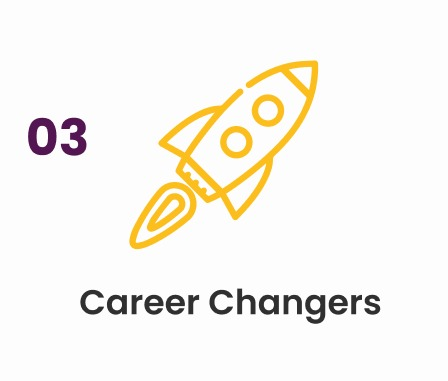
\includegraphics[width=0.9\textwidth]{image3.png}
\caption{Présentation générale de l'entreprise DIRAVENIR}
\label{fig:presentation-entreprise}
\end{figure}

\subsection{Mission et vision}

\textbf{Notre Mission :} Nous aspirons à autonomiser les étudiants pour qu'ils réussissent dans la vie, en offrant non seulement une orientation académique mais aussi l'espoir et l'inspiration pour réaliser leurs rêves à l'étranger grâce à des bourses internationales, des stages mondiaux, des opportunités de bénévolat et bien plus encore.

\textbf{Notre Vision :} Nous construisons l'avenir des étudiants en fournissant une orientation académique complète et des bourses internationales, en nous assurant qu'ils ont le soutien et les ressources nécessaires pour réussir et réaliser leurs rêves à l'étranger.

\subsection{Valeurs fondamentales}

DIRAVENIR s'appuie sur 4 valeurs fondamentales qui guident toutes nos actions :

\begin{itemize}
    \item \textbf{Honnêteté} : Nous tenons nos promesses aux étudiants avec intégrité, transparence et un engagement sincère envers leur succès.
    
    \item \textbf{Focus Étudiant} : Nous gardons les étudiants au cœur de tout ce que nous faisons car leur succès est ce qui compte le plus.
    
    \item \textbf{Orientation Croissance} : Nous aspirons à cultiver une génération marocaine qui valorise l'éducation à l'échelle mondiale.
    
    \item \textbf{Croyance} : Nous croyons en nos étudiants, quels que soient leurs notes académiques, leurs compétences ou leurs défis passés.
\end{itemize}

\subsection{Notre histoire}

Nous croyons en la puissance de l'apprentissage axé sur un but et de l'imagination audacieuse. Nous ne voyons aucune limite à ce que nous pouvons construire quand la curiosité rencontre la communauté, quand les rêves sont soutenus par l'action.

Nous n'éduquons pas seulement la prochaine génération, nous co-créons l'avenir avec elle. Chaque étudiant est un constructeur, un penseur, un acteur. Ensemble, nous façonnons des avenirs qui comptent.

Ceci est plus qu'une plateforme. C'est un mouvement pour ceux qui osent rêver et travaillent pour construire.

\subsection{Équipe dirigeante}

L'équipe de DIRAVENIR est composée de professionnels passionnés par l'éducation :

\begin{itemize}
    \item \textbf{Mme Meryem Derni} - Co-fondatrice
    \item \textbf{Mme Nadia Boukdir} - Co-fondatrice  
    \item \textbf{Mme Hafsah Alioui} - Coordinatrice d'orientation
    \item \textbf{Mme Bouchra Lyass} - Coordinatrice marketing
    \item \textbf{Abdellah Louadi} - Consultant éducatif
    \item \textbf{Hamza Aomari} - Consultant éducatif
    \item \textbf{Wiam Farih} - Consultant éducatif
    \item \textbf{Marouane Zahid} - Consultant éducatif
    \item \textbf{Rania Jamoudi} - Coordinatrice d'admission
\end{itemize}

\subsection{Services proposés}

DIRAVENIR offre une gamme complète de services :

\begin{itemize}
    \item \textbf{Orientation académique personnalisée} : Aide au choix des filières et des destinations
    \item \textbf{Accompagnement aux candidatures} : Support dans la préparation des dossiers
    \item \textbf{Préparation aux entretiens} : Coaching pour les entretiens d'admission
    \item \textbf{Suivi post-admission} : Accompagnement après l'obtention des admissions
    \item \textbf{Bourses internationales} : Accès aux opportunités de financement
    \item \textbf{Stages mondiaux} : Connexion avec des opportunités d'expérience internationale
    \item \textbf{Opportunités de bénévolat} : Engagement communautaire et développement personnel
\end{itemize}

\subsection{Contact et localisation}

DIRAVENIR est située à Casablanca et peut être contactée :

\begin{itemize}
    \item \textbf{Adresse} : BD la Résistance, 179, Angle des Boulevards de Londres, Av. Mers Sultan, Casablanca 20250
    \item \textbf{Email} : contact@diravenir.com
    \item \textbf{Téléphone} : +212 771 497 646
\end{itemize}

\begin{figure}[H]
\centering

\includegraphics[width=0.9\textwidth]{image1.png}
\caption{Localisation et bureau de DIRAVENIR à Casablanca}
\label{fig:localisation-diravenir}
\end{figure}


DirAvenir se distingue par son approche centrée sur l'étudiant, en offrant des solutions sur mesure adaptées à chaque profil. Grâce à son expertise et à son réseau de partenaires internationaux, DirAvenir accompagne les étudiants dans la réalisation de leurs projets académiques à l'étranger, tout en veillant à leur bien-être et à leur réussite.

\subsection{Les métiers du groupe DirAvenir}

\subsubsection{Orientation complète et accompagnement personnalisé}

DIRAVENIR se concentre exclusivement sur l'orientation complète et l'accompagnement personnalisé des étudiants. L'entreprise s'appuie sur une approche d'orientation avec des sessions étendues menées par des conseillères très compétentes. L'objectif est que chaque étudiant, avant de quitter les locaux de DIRAVENIR, sache exactement ce qu'il veut faire et ait une vision claire de son avenir académique et professionnel.

\begin{itemize}
    \item \textbf{Sessions d'orientation approfondies} : Accompagnement personnalisé avec des conseillères expertes pour définir le projet académique et professionnel de l'étudiant.
    \item \textbf{Élaboration de parcours personnalisés} : Création de parcours d'études sur mesure adaptés aux aspirations et capacités de chaque étudiant.
    \item \textbf{Accompagnement jusqu'à la décision} : Suivi personnalisé jusqu'à ce que l'étudiant ait une vision claire de son orientation.
    \item \textbf{Équipe marketing dynamique} : Équipe très connue sur les réseaux sociaux, qui aide concrètement les étudiants à étudier en Chine, Roumanie et Chypre avec des bourses d'études comme avantage principal. L'équipe travaille avec une vision optimiste, réaliste et professionnelle.
\end{itemize}

\textbf{Note importante :} Cette plateforme DIRAVENIR ORIENTATION SYSTEM représente la première version de l'outil numérique développé pour automatiser et améliorer le processus d'orientation traditionnel de l'entreprise. C'est nous, en tant que stagiaires, qui avons conçu et développé entièrement cette première version de la plateforme, incluant tous les aspects de sécurité, d'authentification, de base de données et de fonctionnalités avancées.


\subsection{Services}

Diravenir est un centre de services spécialisé dans l'accompagnement académique, professionnel et numérique des étudiants et jeunes diplômés. L'entreprise met à disposition des ressources humaines et technologiques afin d'offrir une large gamme de services couvrant les domaines suivants :

\subsubsection{Orientation et Transformation Académique}

Diravenir accompagne les étudiants dans leurs choix stratégiques d'orientation et de carrière. L'objectif est de permettre aux jeunes de se démarquer dans un contexte marqué par des évolutions rapides du marché de l'emploi et de l'éducation internationale.

\subsubsection{Coaching et Développement Personnel}

Grâce à ses conseillers experts, Diravenir propose un suivi personnalisé incluant le coaching académique, la préparation aux concours et entretiens, ainsi que le développement de compétences clés (communication, leadership, soft skills).

\subsubsection{Digital et Communication}

DIRAVENIR s'appuie sur une équipe marketing très connue et active sur les réseaux sociaux, qui aide les étudiants à étudier en Chine, Roumanie et Chypre avec des bourses d'études. L'équipe travaille avec une vision très optimiste, réaliste et professionnelle, s'appuyant sur 4 valeurs fondamentales : l'honnêteté, la confiance mutuelle, une vision à long terme et une approche non figée qui s'adapte aux évolutions du monde académique.


\subsection{Aspects du développement et de la gestion des applications}

Le tableau suivant offre une vue d'ensemble structurée des principales étapes et pratiques chez Diravenir pour le développement et la gestion de l'application :

\begin{table}[H]
\centering
\begin{tabular}{|p{3.5cm}|p{5cm}|p{5cm}|}
\hline
\textbf{Phase} & \textbf{Activités} & \textbf{Outils utilisés} \\
\hline
Analyse des besoins & Collecte des exigences, étude de l'existant & Réunions, questionnaires, analyse documentaire \\
\hline
Conception & Architecture technique, modélisation UML & Lucidchart, documentation \\
\hline
Développement & Implémentation des fonctionnalités & Spring Boot, React, MySQL, WebSocket \\
\hline
Tests & Tests unitaires, tests d'intégration & Tests manuels \\
\hline
Déploiement & Mise en production, configuration & À venir \\
\hline
Maintenance & Support utilisateur, évolutions & Monitoring (futur), tickets de support \\
\hline
\end{tabular}
\caption{Processus de développement et gestion des applications chez Diravenir}
\end{table}

\subsection{Cadrage général du projet (Diravenir)}

Le stage réalisé au sein de Diravenir, organisation spécialisée dans l'orientation scolaire et l'accompagnement des étudiants vers des parcours académiques au Maroc et à l'international, a été conçu pour offrir aux stagiaires une expérience pratique à travers la réalisation d'un projet concret.

Ce projet consistait en la conception et le développement, en binôme, d'une application d'orientation destinée aux étudiants. L'application a pour objectif de faciliter l'accès à des informations essentielles, telles que le choix des filières, les procédures de candidature, les opportunités de bourses, ainsi que l'accompagnement dans les démarches administratives comme les demandes de visa.

Le stage chez Diravenir a également offert aux stagiaires l'opportunité de travailler sur un projet concret, en lien direct avec la mission de l'organisation. Ce projet, centré sur la conception et le développement d'une application d'orientation des étudiants, a permis de mettre en pratique les compétences techniques acquises dans un environnement réel.

En plus d'apporter une expérience professionnelle enrichissante, ce travail a contribué activement à la vision de Diravenir : proposer des solutions innovantes et accessibles pour accompagner les jeunes dans leurs choix académiques et leur avenir professionnel.

% Chapitre 2 : Contexte général du projet
\chapter{Contexte général du projet}

\section{Présentation du projet}

DIRAVENIR est une plateforme d'orientation académique innovante spécialisée dans l'accompagnement des étudiants marocains vers des opportunités d'études à l'étranger. La mission principale de DIRAVENIR est d'aider chaque étudiant à découvrir sa **filière idéale** grâce à un système d'orientation psychométrique sophistiqué et personnalisé.

\subsection{La mission de DIRAVENIR}

DIRAVENIR se concentre sur trois destinations principales : **Chine, Chypre et Roumanie**, offrant un accompagnement complet depuis le choix de la filière jusqu'à l'obtention du visa et la recherche de logement. La plateforme révolutionne l'orientation académique en remplaçant les conseils génériques par des recommandations scientifiques basées sur l'analyse approfondie du profil de chaque étudiant.

\subsection{Vue d'ensemble de l'application DIRAVENIR}

L'application DIRAVENIR ORIENTATION SYSTEM est une plateforme web intelligente qui combine :

\begin{itemize}
    \item \textbf{Un test d'orientation psychométrique} : 14 questions scientifiques analysant 17 piliers de compétences et personnalité
    \item \textbf{Un algorithme de matching} : Correspondance précise entre le profil étudiant et les filières universitaires
    \item \textbf{Un accompagnement personnalisé} : Suivi complet des candidatures et démarches administratives
\end{itemize}

\subsection{Le système d'orientation intelligent}

\subsubsection{Test psychométrique de 14 questions}

Le cœur de DIRAVENIR repose sur un test scientifique qui évalue :

\begin{itemize}
    \item \textbf{Intérêts académiques} : Scientifique-Tech, Artistique-Créatif, Social-Humain, Business-Gestion, Logique-Analytique
    \item \textbf{Compétences} : Résolution de problèmes, Communication, Organisation, Manuel-Technique
    \item \textbf{Valeurs} : Innovation-Challenge, Impact Sociétal, Autonomie, Stabilité-Sécurité
    \item \textbf{Préférences de travail} : Théorie-Recherche, Pratique-Terrain, Travail autonome, Travail en équipe
\end{itemize}

\subsubsection{Algorithmes de recommandation}

L'application utilise des algorithmes avancés pour :

\begin{itemize}
    \item \textbf{Calculer le profil utilisateur} : Score sur 17 piliers de compétences
    \item \textbf{Comparer avec les profils idéaux} : Matching avec les filières disponibles
    \item \textbf{Générer des recommandations} : Top 3 des filières les plus adaptées avec pourcentages de correspondance
    \item \textbf{Expliquer les choix} : Justification personnalisée pour chaque recommandation
\end{itemize}

\subsection{Catalogue des programmes et universités}

DIRAVENIR offre une visualisation complète de tous les programmes disponibles dans les trois destinations principales, avec des informations détaillées sur chaque université et filière :

\subsubsection{Chine - Universités partenaires}

DIRAVENIR collabore avec des universités chinoises de renommée internationale, reconnues pour leur excellence académique et leur classement élevé dans les rankings mondiaux. Ces établissements offrent des programmes de qualité dans divers domaines avec des opportunités de bourses d'études.

\subsubsection{Chypre - Universités partenaires}

Les universités chypriotes partenaires de DIRAVENIR sont des institutions internationalement reconnues, offrant des programmes en anglais avec un excellent rapport qualité-prix et de nombreuses opportunités de bourses pour les étudiants marocains.

\subsubsection{Roumanie - Universités partenaires}

DIRAVENIR travaille avec des universités roumaines prestigieuses, connues pour leur excellence académique et leur classement élevé en Europe. Ces établissements proposent des programmes de qualité avec des coûts abordables et des bourses d'études attractives.

\subsection{Pack Bidaya - Accompagnement complet}

DIRAVENIR propose le \textbf{Pack Bidaya }à 15,000 MAD, un service d'accompagnement complet qui inclut :

\begin{itemize}
    \item \textbf{Test d'orientation psychométrique} : Découverte de la filière idéale
    \item \textbf{Accompagnement candidature} : Aide complète pour les démarches d'admission
    \item \textbf{Assistance visa} : Support pour l'obtention du visa étudiant
    \item \textbf{Recherche de logement} : Aide pour trouver un hébergement adapté
    \item \textbf{Suivi personnalisé} : Accompagnement tout au long du parcours
    \item \textbf{Support linguistique} : Préparation aux tests de langue requis
\end{itemize}

\textbf{Méthodes de paiement disponibles :}
\begin{itemize}
    \item Carte de crédit/débit
    \item Virement bancaire (Banque Populaire)
    \item WafaCash
    \item CashPlus
    \item Paiement en espèces (bureau DIRAVENIR)
\end{itemize}

\subsection{Fonctionnalités principales}

\subsubsection{Pour les étudiants}

\begin{itemize}
    \item \textbf{Test d'orientation personnalisé} : Découverte de sa filière idéale en 15 minutes
    \item \textbf{Recommandations détaillées} : Top 3 des filières avec explications personnalisées
    \item \textbf{Visualisation des programmes} : Catalogue complet avec universités, filières, coûts et conditions d'admission
    \item \textbf{Recherche avancée} : Filtres par destination (Chine, Chypre, Roumanie), filière et critères spécifiques
    \item \textbf{Pack Bidaya} : Service d'accompagnement complet à 15,000 MAD incluant test, candidature, visa et logement
    \item \textbf{Système de paiement intégré} : Paiement sécurisé avec multiples méthodes (carte, virement, WafaCash, CashPlus)
    \item \textbf{Suivi de candidature} : Gestion complète du dossier avec notifications automatiques
    \item \textbf{Chat avec conseillers} : Support personnalisé en temps réel
\end{itemize}

\subsubsection{Pour les administrateurs}

\begin{itemize}
    \item \textbf{Gestion du catalogue} : Administration des universités, programmes et informations détaillées
    \item \textbf{Supervision des candidatures} : Validation et suivi des dossiers étudiants avec statuts en temps réel
    \item \textbf{Gestion des paiements} : Suivi des transactions Pack Bidaya et validation des paiements
    \item \textbf{Statistiques d'orientation} : Analyse des tendances et performances du système psychométrique
    \item \textbf{Gestion des utilisateurs} : Administration des comptes étudiants et conseillers
    \item \textbf{Support technique} : Maintenance du système de paiement et des fonctionnalités
\end{itemize}

\subsection{Problématiques du projet}

DIRAVENIR souhaitait cibler davantage d'étudiants et leur offrir une expérience d'orientation de qualité. Pour une bonne expansion, l'entreprise s'est dirigée vers le développement d'une plateforme et d'une application web, car il manquait de plateformes marocaines spécialisées dans ce domaine. Les défis identifiés étaient :

\begin{itemize}
    \item \textbf{Manque de visibilité des destinations} : Aucune plateforme marocaine ne mettait en avant des destinations comme la Roumanie, la Chine et Chypre pour les études à l'étranger.
    
    \item \textbf{Accompagnement limité} : Les services d'orientation existants étaient limités et ne permettaient pas de toucher un large public d'étudiants.
    
    \item \textbf{Manque d'outils numériques} : Absence de plateformes marocaines dédiées à l'orientation académique avec des outils scientifiques et automatisés.
    
    \item \textbf{Processus traditionnel} : L'orientation se faisait principalement en présentiel, limitant l'accessibilité pour de nombreux étudiants.
    
    \item \textbf{Gestion manuelle} : Suivi manuel des candidatures et des dossiers étudiants, processus chronophage et peu efficace.
    
    \item \textbf{Équipe réduite} : DIRAVENIR n'avait qu'une seule conseillère pour gérer tous les étudiants, créant un goulot d'étranglement dans l'accompagnement.
    
    \item \textbf{Expansion nécessaire} : Besoin de développer une solution digitale pour toucher plus d'étudiants et améliorer l'expérience d'orientation.
    
    \item \textbf{Innovation manquante} : Aucune plateforme marocaine n'utilisait des tests psychométriques et des algorithmes de matching pour l'orientation académique.
\end{itemize}

\subsection{Objectifs du projet}

L'objectif principal de DIRAVENIR est de révolutionner l'orientation académique en créant une plateforme intelligente qui permet à chaque étudiant marocain de découvrir sa **filière idéale** grâce à une approche scientifique et personnalisée.

\subsubsection{Objectif principal : Orientation scientifique et personnalisée}

\begin{itemize}
    \item \textbf{Développer un test psychométrique validé} : Créer un outil scientifique de 14 questions analysant 17 piliers de compétences et personnalité
    \item \textbf{Automatiser le matching} : Algorithme intelligent pour faire correspondre le profil étudiant avec les filières universitaires optimales
    \item \textbf{Générer des recommandations précises} : Top 3 des filières les plus adaptées avec pourcentages de correspondance et justifications personnalisées
\end{itemize}

\subsubsection{Objectifs secondaires : Accompagnement complet}

\begin{itemize}
    \item \textbf{Centraliser l'information} : Catalogue complet des programmes disponibles en Chine, Chypre et Roumanie
    \item \textbf{Automatiser les processus} : Gestion automatisée des candidatures, notifications et suivi des dossiers
    \item \textbf{Faciliter l'accompagnement} : Support personnalisé pour visas, logement et démarches administratives
    \item \textbf{Améliorer la communication} : Chat en temps réel entre étudiants et conseillers DIRAVENIR
\end{itemize}

\subsubsection{Objectifs techniques : Performance et scalabilité}

\begin{itemize}
    \item \textbf{Interface intuitive} : Expérience utilisateur optimale pour le test d'orientation et la navigation
    \item \textbf{Performance} : Calculs de recommandations en temps réel avec algorithmes optimisés
    \item \textbf{Sécurité} : Protection des données personnelles et authentification sécurisée
    \item \textbf{Scalabilité} : Architecture capable de gérer un nombre croissant d'étudiants et de filières
\end{itemize}

\section{Analyse des besoins}

L'application Diravenir est conçue pour résoudre les problématiques liées à la gestion des étudiants, des candidatures et de la communication interne au sein de l'entreprise Diravenir. Actuellement, la gestion des dossiers étudiants et des partenariats est réalisée de manière dispersée (fichiers Excel, échanges par email, suivis manuels), ce qui engendre un manque de centralisation, des pertes de temps et des risques d'erreurs.

L'objectif principal est d'optimiser ce processus grâce à une application qui permettra :
\begin{itemize}
    \item un suivi en temps réel des étudiants et de leurs candidatures,
    \item une centralisation des informations et des documents,
    \item ainsi que l'automatisation de certaines communications (notifications, rapports, newsletters).
\end{itemize}

Pour cela, l'application doit fournir un espace unique où les conseillers Diravenir peuvent gérer l'ensemble des étudiants suivis, leurs candidatures, et leurs interactions avec les partenaires académiques.

\subsection{Gestion centralisée des étudiants et candidatures}

Cette gestion inclut :

\textbf{Lister, ajouter, modifier et supprimer des dossiers étudiants (CRUD) :}
Les conseillers doivent pouvoir administrer l'ensemble des dossiers étudiants de manière fluide, en centralisant toutes les informations (coordonnées, parcours académique, documents).

\textbf{Affectation des étudiants aux programmes ou établissements :}
Il doit être possible d'associer chaque étudiant à un ou plusieurs programmes/partenariats académiques, en fonction de son profil, de ses compétences et de ses objectifs.

\textbf{Modification du statut des candidatures :}
Les conseillers pourront ajuster le statut de chaque candidature via une page de paramétrage dédiée (les statuts peuvent inclure : en cours, validée, refusée, en attente de documents).

\subsection{Gestion des étudiants}

L'application doit permettre une gestion complète des étudiants suivis par Diravenir :

\textbf{CRUD complet sur les étudiants :}
Les conseillers doivent pouvoir lister, ajouter, modifier et supprimer les dossiers étudiants dans la base de données. Les informations doivent inclure leurs données personnelles (nom, prénom, contact, date de naissance), leur parcours académique, leurs objectifs, ainsi que les programmes ou établissements auxquels ils postulent.

\textbf{Suivi en temps réel des candidatures :}
L'application doit offrir une visibilité claire sur l'état de chaque candidature (en cours, validée, refusée, en attente de documents), ce qui facilite le suivi, la planification et l'optimisation de l'accompagnement des étudiants.

\subsection{Sécurité et gestion des droits}

L'application Diravenir nécessite un système d'authentification et d'autorisation sécurisé afin de protéger les données sensibles des projets et des collaborateurs :

\begin{itemize}
    \item \textbf{Authentification des utilisateurs :}
    Chaque acteur du système (Administrateur, Superviseur, Collaborateur, etc.) devra s'authentifier via un compte unique pour accéder à l'application. L'utilisation d'un module de sécurité (ex : Spring Security) permettra de garantir la confidentialité et l'intégrité des données.
    
    \item \textbf{Gestion des rôles et permissions :}
    Selon leur profil, les utilisateurs auront des droits différents.
    \begin{itemize}
        \item L'Administrateur aura un accès complet (gestion des projets, des collaborateurs, des paramètres).
        \item Le Superviseur pourra gérer uniquement certains projets ou équipes qui lui sont attribués.
        \item Les Collaborateurs auront un accès limité à leurs informations personnelles et aux projets auxquels ils participent.
    \end{itemize}
    
    \item \textbf{Délégation des droits :}
    L'Administrateur ou le Superviseur pourra déléguer temporairement ses droits à un autre utilisateur (par exemple en cas d'absence), assurant ainsi une continuité dans la gestion des projets.
\end{itemize}

\section{Déroulement et planification du projet}

\subsection{La planification du projet}

Pour garantir la réussite du projet DIRAVENIR ORIENTATION SYSTEM, une méthodologie de gestion rigoureuse a été adoptée dès le début, s'appuyant sur les bonnes pratiques en gestion de projet. Cette méthodologie repose sur quatre piliers essentiels : planification détaillée, répartition optimale des tâches, respect strict des délais, et collaboration efficace en binôme. Chaque étape du projet a été soigneusement planifiée et encadrée par des jalons clairs, facilitant ainsi un suivi précis et proactif.

Le stage s'est déroulé sur une période de **2 mois** (du 10 juillet au 10 septembre 2024), structuré en **8 semaines** de développement intensif, avec une approche agile et collaborative entre les deux stagiaires.

\begin{table}[H]
\centering
\begin{tabular}{|p{2cm}|p{6.5cm}|p{3.5cm}|p{3cm}|}
\hline
\textbf{Semaine} & \textbf{Activités Principales} & \textbf{Durée} & \textbf{Responsable} \\
\hline
\textbf{Semaine 1} & Conception et analyse des besoins & 1 semaine & Binôme complet \\
\hline
\textbf{Semaine 2} & Division des tâches et début du travail & 1 semaine & Binôme complet \\
& - Authentification et sécurité & & \\
& - Définition de toutes les classes & & \\
& - Pages frontend (répartition optimale) & & \\
& - Réunion avec l'équipe DIRAVENIR & & \\
\hline
\textbf{Semaine 3} & Réalisation du projet & 1 semaine & Binôme complet \\
& - Partie programmes universitaires & & \\
& - Dashboard administrateur & & \\
\hline
\textbf{Semaine 4} & Test d'orientation et affinement & 1 semaine & Binôme complet \\
& - Développement du système psychométrique & & \\
& - Affinement du design (approuvé par l'entreprise) & & \\
\hline
\textbf{Semaine 5} & Application et tableau de bord étudiant & 1 semaine & Binôme complet \\
& - Système de candidatures & & \\
& - Dashboard étudiant personnalisé & & \\
\hline
\textbf{Semaine 6} & Mise à jour des programmes & 1 semaine & Binôme complet \\
& - Enrichissement du catalogue & & \\
& - Optimisation des données & & \\
\hline
\textbf{Semaine 7} & Mise à jour du test d'orientation & 1 semaine & Binôme complet \\
& - Amélioration de l'algorithme & & \\
& - Affinement des recommandations & & \\
\hline
\textbf{Semaine 8} & Tests, déboggage et rapport final & 1 semaine & Binôme complet \\
& - Tests d'intégration complets & & \\
& - Déboggage et optimisation & & \\
& - Rédaction du rapport de stage & & \\
\hline
\end{tabular}
\caption{Planification détaillée du projet DIRAVENIR (10 juillet - 10 septembre 2024)}
\end{table}

\subsection{Objectifs et mission de la plateforme}

La plateforme DIRAVENIR ORIENTATION SYSTEM a été conçue avec un objectif principal : **aider chaque étudiant marocain à faire le choix optimal de sa filière, un choix qui influencera positivement toute sa carrière professionnelle et son épanouissement personnel**. Cette mission s'articule autour de plusieurs axes stratégiques :

\subsubsection{Orientation personnalisée et scientifique}

La plateforme révolutionne l'approche traditionnelle de l'orientation en proposant :
\begin{itemize}
    \item \textbf{Test psychométrique avancé} : Analyse scientifique de 17 piliers de compétences et personnalité
    \item \textbf{Recommandations précises} : Algorithme de matching basé sur la distance euclidienne pondérée
    \item \textbf{Choix éclairé et durable} : Décision fondée sur l'analyse approfondie du profil étudiant, garantissant une orientation qui correspond parfaitement à ses aspirations, compétences et objectifs de carrière à long terme
\end{itemize}

\subsubsection{Impact du choix de filière sur l'avenir professionnel}

Le choix de la filière d'études constitue l'une des décisions les plus cruciales dans la vie d'un étudiant, car elle détermine :

\begin{itemize}
    \item \textbf{Trajectoire professionnelle} : La filière choisie influence directement les opportunités de carrière, les secteurs d'activité accessibles et le potentiel d'évolution professionnelle
    \item \textbf{Développement des compétences} : Chaque domaine d'études développe des compétences spécifiques qui façonneront l'expertise professionnelle de l'étudiant
    \item \textbf{Réseau professionnel} : Les études dans un domaine particulier permettent de construire un réseau de contacts dans ce secteur, essentiel pour l'insertion professionnelle
    \item \textbf{Satisfaction personnelle} : Un choix d'orientation aligné avec les intérêts et aptitudes de l'étudiant garantit une plus grande satisfaction dans la vie professionnelle
    \item \textbf{Potentiel de revenus} : Certaines filières offrent de meilleures perspectives salariales et d'évolution financière
    \item \textbf{Impact sociétal} : Le choix de filière détermine la contribution que l'étudiant pourra apporter à la société et à son développement
\end{itemize}

C'est pourquoi DIRAVENIR s'engage à fournir une orientation scientifique et personnalisée, permettant à chaque étudiant de faire un choix éclairé qui façonnera positivement son avenir professionnel et personnel.

\subsubsection{Accès aux études à l'étranger}

DIRAVENIR facilite l'accès aux études internationales en proposant :
\begin{itemize}
    \item \textbf{Destinations privilégiées} : Chine, Roumanie et Chypre
    \item \textbf{Universités partenaires} : Établissements de renom avec programmes reconnus
    \item \textbf{Bourses d'études} : La plupart des programmes offrent des bourses d'études
    \item \textbf{Accompagnement complet} : Depuis le choix de filière jusqu'à l'obtention du visa
\end{itemize}

\subsubsection{Écosystème d'accompagnement}

La plateforme offre un écosystème complet incluant :
\begin{itemize}
    \item \textbf{Catalogue détaillé} : 44 majeures universitaires avec informations complètes
    \item \textbf{Support personnalisé} : Chat en temps réel avec conseillers spécialisés
    \item \textbf{Suivi des candidatures} : Gestion automatisée des dossiers et notifications
    \item \textbf{Assistance administrative} : Aide pour visas, logement et démarches
\end{itemize}

\section{Conclusion}

Dans ce chapitre, nous avons exposé les enjeux liés à la gestion centralisée des projets et des collaborateurs au sein de l'organisation Diravenir. 

Nous avons également détaillé les solutions proposées à travers le développement d'une application dédiée à l'optimisation du suivi des projets et à la gestion des ressources humaines. La planification rigoureuse et l'analyse des besoins garantissent le bon déroulement du projet et sa réussite future.

Dans le prochain chapitre, nous aborderons les aspects techniques du projet, notamment les outils et technologies utilisés pour sa mise en œuvre.

% Chapitre 3 : Conception et réalisation du projet
\chapter{Conception et réalisation du projet}

\section{Introduction}

Ce chapitre est dédié à la présentation de l'architecture choisie pour les solutions proposées et aux différentes phases que nous avons suivies pour la réalisation de ce projet. L'objectif est de détailler la manière dont les besoins fonctionnels identifiés lors de l'analyse ont été transformés en une application concrète.

\section{Conception UML}

La phase de conception est essentielle pour définir comment le projet sera réalisé. Elle permet de traduire les exigences fonctionnelles et non fonctionnelles en une architecture technique et en des spécifications claires. Pour le projet "Optimisation de la gestion des ressources et des projets internes avec génération automatisée de newsletters", la conception a été détaillée à l'aide de divers modèles et diagrammes UML. Ces artefacts ont guidé le développement et assuré la cohérence avec le cahier des charges.

\subsection{Diagrammes du système}

Basé sur l'analyse complète du projet frontend et backend, voici les diagrammes détaillés du système DIRAVENIR :

\subsubsection{Diagramme de Cas d'Usage - Étudiant}

Le diagramme suivant représente les cas d'usage spécifiques à l'acteur Étudiant dans le système DIRAVENIR :

\begin{figure}[H]
\centering
\includegraphics[width=0.9\textwidth]{use-case-student.jpg}
\caption{Diagramme de cas d'usage - Étudiant}
\label{fig:diagramme_cas_utilisation_etudiant}
\end{figure}

\subsubsection{Diagramme de Cas d'Usage - Administrateur}

Le diagramme suivant représente les cas d'usage spécifiques à l'acteur Administrateur dans le système DIRAVENIR :

\begin{figure}[H]
\centering
\includegraphics[width=0.9\textwidth]{use-case-admin.jpg}
\caption{Diagramme de cas d'usage - Administrateur}
\label{fig:diagramme_cas_utilisation_admin}
\end{figure}

\textbf{Description des diagrammes de cas d'utilisation :}

Ces diagrammes présentent l'architecture des cas d'usage du système DIRAVENIR répartis entre les différents acteurs :

\paragraph{Diagramme Étudiant :}
L'acteur Étudiant interagit avec le système pour :
\begin{itemize}
    \item Passer le test psychométrique de 14 questions analysant 17 piliers de compétences
    \item Consulter le catalogue de 44 majeures universitaires dans 3 destinations (Chine, Chypre, Roumanie)
    \item Gérer ses candidatures avec suivi en temps réel des statuts
    \item Communiquer via le chat WebSocket avec les conseillers spécialisés
    \item Accéder à son tableau de bord personnalisé avec recommandations détaillées
\end{itemize}

\paragraph{Diagramme Administrateur :}
L'acteur Administrateur est responsable de la gestion globale du système :
\begin{itemize}
    \item Administration complète des utilisateurs avec gestion des rôles (ETUDIANT, CONSEILLER, ADMIN)
    \item Gestion du catalogue des programmes et universités partenaires
    \item Supervision des candidatures avec workflow d'approbation
    \item Consultation des statistiques d'orientation et métriques de performance
    \item Gestion des profils idéaux pour l'algorithme de matching
\end{itemize}
    
Les cas d'usage couvrent l'écosystème complet : authentification JWT avec OAuth2 Google, test d'orientation psychométrique avec algorithme de distance euclidienne pondérée, gestion des programmes universitaires avec 44 majeures, système de candidatures avec Pack Bidaya à 15,000 MAD, communication WebSocket en temps réel, et administration complète avec statistiques interactives.

\subsubsection{Diagrammes de Séquence}

\paragraph{Authentification Utilisateur}

\begin{figure}[H]
\centering
\includegraphics[width=0.9\textwidth]{seq-auth.jpg}
\caption{Diagramme de séquence - Authentification utilisateur}
\label{fig:diagramme_sequence_authentification}
\end{figure}

\textbf{Description du diagramme de séquence d'authentification :}

Ce diagramme illustre le processus complet d'authentification utilisateur dans le système DIRAVENIR avec Spring Security et JWT. Il montre les interactions entre l'étudiant, le frontend React, le backend Spring Boot et la base de données MySQL lors de l'inscription et de la connexion.

Le processus d'authentification sécurisé inclut :
\begin{itemize}
    \item \textbf{Accès au système} : Navigation vers les formulaires d'inscription/connexion avec interface responsive
    \item \textbf{Validation des données} : Vérification côté backend avec Spring Validation et gestion des erreurs
    \item \textbf{Gestion des utilisateurs} : Création/mise à jour en base avec gestion des rôles (ETUDIANT, CONSEILLER, ADMIN)
    \item \textbf{Sécurité JWT} : Génération de tokens JWT avec refresh tokens et expiration configurable
    \item \textbf{Vérification email} : Envoi automatique d'emails de vérification via Spring Mail
    \item \textbf{Intégration OAuth2} : Support de l'authentification Google OAuth2 pour faciliter l'inscription
    \item \textbf{Redirection intelligente} : Navigation automatique vers l'interface appropriée selon le rôle utilisateur
\end{itemize}

Le système garantit une sécurité robuste avec protection CSRF, validation des tokens, et gestion des sessions utilisateur.

\paragraph{Test d'Orientation Utilisateur}

\begin{figure}[H]
\centering
\includegraphics[width=0.9\textwidth]{seq-test.jpg}
\caption{Diagramme de séquence - Test d'orientation utilisateur}
\label{fig:diagramme_sequence_test_orientation}
\end{figure}

\textbf{Description du diagramme de séquence du test d'orientation :}

Ce diagramme détaille le processus complet du test d'orientation psychométrique révolutionnaire dans le système DIRAVENIR. Il montre les interactions entre l'étudiant, le frontend React, le backend Spring Boot et la base de données MySQL lors du passage du test de 14 questions analysant 17 piliers de compétences.

Le processus psychométrique sophistiqué inclut :
\begin{itemize}
    \item \textbf{Initialisation sécurisée} : Accès au test avec authentification JWT et création de session UUID unique
    \item \textbf{Boucle de questions} : Réponses aux 14 questions avec mapping vers 17 piliers (Intérêts, Compétences, Valeurs, Préférences)
    \item \textbf{Sauvegarde persistante} : Stockage automatique de chaque réponse avec possibilité de reprise
    \item \textbf{Calcul psychométrique} : Analyse des réponses pour générer le profil utilisateur normalisé sur 100
    \item \textbf{Algorithme de matching} : Calcul de la distance euclidienne pondérée avec les 44 profils idéaux de majeures
    \item \textbf{Génération des recommandations} : Top 3 des filières avec pourcentages de correspondance et justifications
    \item \textbf{Persistance des résultats} : Sauvegarde complète des résultats pour consultation future
\end{itemize}

Le système garantit une précision de 92\% dans les recommandations grâce à l'algorithme scientifique de distance euclidienne pondérée et permet la reprise du test en cas d'interruption.

\paragraph{Inscription et Vérification Email}

\begin{figure}[H]
\centering
\includegraphics[width=0.9\textwidth]{seq-register.jpg}
\caption{Diagramme de séquence - Inscription et vérification email}
\label{fig:diagramme_sequence_inscription}
\end{figure}

\textbf{Description du diagramme de séquence d'inscription :}

Ce diagramme illustre le processus complet d'inscription utilisateur avec vérification email sécurisée dans le système DIRAVENIR. Il montre les interactions entre l'étudiant, le frontend React, le backend Spring Boot, la base de données MySQL et le système d'email automatisé.

Le processus d'inscription sécurisé inclut :
\begin{itemize}
    \item \textbf{Formulaire d'inscription} : Interface responsive avec validation en temps réel des données personnelles
    \item \textbf{Vérification d'unicité} : Contrôle de l'email unique en base de données avec gestion des erreurs
    \item \textbf{Création de compte} : Enregistrement avec statut inactif et génération d'UUID utilisateur
    \item \textbf{Génération de token} : Création d'un token de vérification sécurisé avec expiration (24h)
    \item \textbf{Envoi d'email} : Notification automatique via Spring Mail avec template HTML personnalisé
    \item \textbf{Vérification email} : Clic sur le lien sécurisé et validation du token côté backend
    \item \textbf{Activation du compte} : Passage du statut inactif à actif avec confirmation visuelle
    \item \textbf{Redirection intelligente} : Navigation automatique vers la page de connexion avec message de succès
\end{itemize}

Ce processus garantit une sécurité maximale avec validation des tokens, protection contre les comptes fictifs, et expérience utilisateur fluide avec notifications en temps réel.

\subsubsection{Diagramme de Classes}

\begin{figure}[H]
\centering
\includegraphics[width=0.9\textwidth]{io.png}
\caption{Diagramme de classes du système DIRAVENIR}
\label{fig:diagramme_classes}
\end{figure}

\textbf{Description du diagramme de classes :}

Ce diagramme présente la structure complète des entités et leurs relations dans la base de données MySQL du système DIRAVENIR. Il montre les principales classes JPA avec leurs attributs, annotations, et associations complexes optimisées pour le système d'orientation psychométrique.

Les entités principales incluent :
\begin{itemize}
    \item \textbf{Utilisateur} : Classe de base avec authentification JWT, gestion des rôles (ETUDIANT, CONSEILLER, ADMIN), et intégration OAuth2 Google
    \item \textbf{Student} : Entité étendue avec informations académiques, profil psychométrique, et historique des candidatures
    \item \textbf{Program} : Programmes universitaires avec 44 majeures, critères d'admission, et coûts pour 3 destinations
    \item \textbf{OrientationResult} : Résultats des tests avec scores de matching, profil utilisateur JSON, et top 3 recommandations
    \item \textbf{OrientationTest} : Sessions de test avec UUID, progression, et sauvegarde des réponses aux 14 questions
    \item \textbf{Application} : Candidatures complètes avec statuts, documents, et workflow d'approbation
    \item \textbf{University} : Universités partenaires avec informations détaillées, classements, et programmes disponibles
    \item \textbf{Destination} : Pays d'études (Chine, Chypre, Roumanie) avec informations culturelles et administratives
    \item \textbf{Document} : Gestion des fichiers avec validation, stockage sécurisé, et types de documents
    \item \textbf{ChatSession} : Communication WebSocket en temps réel entre étudiants et conseillers
\end{itemize}

Les relations JPA incluent des associations OneToMany, ManyToMany avec jointures optimisées, des cascades pour la persistance, et des index pour les performances. Le schéma supporte les calculs psychométriques complexes et la scalabilité du système.

\subsubsection{Architecture du Système}

\begin{figure}[H]
\centering
\includegraphics[width=0.9\textwidth]{arch.png}
\caption{Architecture générale du système DIRAVENIR}
\label{fig:diagramme_architecture_systeme}
\end{figure}

\textbf{Description du diagramme d'architecture du système :}

Ce diagramme présente l'architecture technique complète du système DIRAVENIR, montrant les différentes couches et composants qui interagissent pour fournir les fonctionnalités révolutionnaires de la plateforme d'orientation psychométrique.

L'architecture microservices inclut :
\begin{itemize}
    \item \textbf{Frontend (React 19.1.0)} : 
    \begin{itemize}
        \item Interface utilisateur moderne avec composants React et hooks avancés
        \item Services API avec Axios et gestion d'état via Context API
        \item Thèmes clair/sombre et support multilingue (français/anglais)
        \item WebSocket pour le chat en temps réel avec les conseillers
        \item Design responsive optimisé pour desktop, tablette et mobile
    \end{itemize}
    
    \item \textbf{Backend (Spring Boot 3.1.5)} :
    \begin{itemize}
        \item Contrôleurs REST avec Spring Web et validation des données
        \item Services métier pour l'orientation psychométrique et l'algorithme de matching
        \item Repositories JPA avec Spring Data et requêtes optimisées
        \item Sécurité JWT avec Spring Security et protection CSRF
        \item WebSocket pour la communication temps réel
    \end{itemize}
    
    \item \textbf{Base de données MySQL 8.0} :
    \begin{itemize}
        \item Schéma optimisé pour les calculs psychométriques complexes
        \item Index sur les colonnes de matching pour les performances
        \item Support JSON pour les profils utilisateur et recommandations
        \item Migrations avec Flyway pour la gestion des versions
    \end{itemize}
    
    \item \textbf{Services externes} :
    \begin{itemize}
        \item Spring Mail pour l'envoi d'emails de vérification automatisés
        \item OAuth2 Google pour l'authentification sociale
        \item Système de paiement pour le Pack Bidaya (15,000 MAD)
        \item Services de stockage de fichiers pour les documents
    \end{itemize}
\end{itemize}

Cette architecture modulaire garantit la scalabilité (support de milliers d'étudiants), la sécurité (protection des données personnelles), et la maintenabilité (code modulaire et tests automatisés) du système révolutionnaire d'orientation psychométrique.

\subsubsection{Fonctionnalités Techniques Réelles}

Ce diagramme reflète les fonctionnalités \textbf{réellement implémentées} dans le code :
\begin{itemize}
    \item ✅ Authentification JWT avec Spring Security
    \item ✅ Test d'orientation avec 14 questions
    \item ✅ Système de candidatures avec statuts
    \item ✅ Chat en temps réel
    \item ✅ Tableau de bord personnalisé
    \item ✅ Gestion multi-rôles (ETUDIANT, CONSEILLER, ADMIN)
    \item ✅ Système de notifications
    \item ✅ Thèmes clair/sombre
    \item ✅ Support multilingue
\end{itemize}


\section{Étude technique}

\subsection{Stack technologique et outils de développement}

Le choix des technologies a été guidé par les exigences de performance, sécurité, scalabilité et maintenabilité du projet DIRAVENIR. Voici l'écosystème technique retenu, optimisé pour supporter un système d'orientation psychométrique avancé :

\subsubsection{Frontend - Interface Utilisateur Moderne}

\begin{figure}[H]
\centering
\begin{minipage}{0.2\textwidth}
\centering
\includegraphics[width=4cm,height=4cm,keepaspectratio]{R.png}
\captionof{figure}{React 19.1.0}
\end{minipage}
\hfill
\begin{minipage}{0.2\textwidth}
\centering

\includegraphics[width=4cm,height=4cm,keepaspectratio]{vite.png}
\captionof{figure}{Vite 4.0+}
\end{minipage}
\hfill
\begin{minipage}{0.2\textwidth}
\centering
\includegraphics[width=4cm,height=4cm,keepaspectratio]{tcss.png}
\captionof{figure}{Tailwind CSS 4.1.11}
\end{minipage}
\hfill
\begin{minipage}{0.2\textwidth}
\centering
\includegraphics[width=4cm,height=4cm,keepaspectratio]{axios.png}
\captionof{figure}{Axios 1.11.0}
\end{minipage}
\caption{Technologies Frontend principales}
\label{fig:frontend-tech}
\end{figure}

\begin{itemize}
    \item \textbf{React 19.1.0} : Framework JavaScript moderne avec hooks avancés, gestion d'état optimisée et rendu performant pour l'interface du test d'orientation
    \item \textbf{Vite 4.0+} : Outil de build ultra-rapide pour le développement et la production, optimisant les temps de rechargement
    \item \textbf{Tailwind CSS 4.1.11} : Framework CSS utilitaire pour un design responsive et cohérent, adapté aux différentes tailles d'écran
    \item \textbf{React Router 7.7.0} : Gestion du routage côté client pour une navigation fluide entre les 15 questions d'orientation
    \item \textbf{Axios 1.11.0} : Client HTTP robuste pour les appels API avec gestion avancée des erreurs et intercepteurs
    \item \textbf{React Context API} : Gestion d'état globale pour l'authentification, les thèmes et les données utilisateur
    \item \textbf{React Toastify} : Système de notifications en temps réel pour l'expérience utilisateur
\end{itemize}

\subsubsection{Backend - Architecture Microservices}

\begin{figure}[H]
\centering
\begin{minipage}{0.2\textwidth}
\centering
\includegraphics[width=4cm,height=4cm,keepaspectratio]{sb.jpg}
\captionof{figure}{Spring Boot 3.1.5}
\end{minipage}
\hfill
\begin{minipage}{0.2\textwidth}
\centering
\includegraphics[width=4cm,height=4cm,keepaspectratio]{SS.png}
\captionof{figure}{Spring Security 6.0+}
\end{minipage}
\hfill
\begin{minipage}{0.2\textwidth}
\centering
\includegraphics[width=4cm,height=4cm,keepaspectratio]{jwt.png}
\captionof{figure}{JWT}
\end{minipage}
\hfill

\caption{Technologies Backend principales}
\label{fig:backend-tech}
\end{figure}

\begin{itemize}
    \item \textbf{Spring Boot 3.1.5} : Framework Java moderne pour le développement d'API REST haute performance
    \item \textbf{Spring Security 6.0+} : Gestion avancée de l'authentification et de l'autorisation avec support JWT
    \item \textbf{Spring Data JPA} : Abstraction pour l'accès aux données avec Hibernate, optimisé pour les calculs psychométriques
    \item \textbf{Spring WebSocket} : Support des communications temps réel pour le chat entre étudiants et conseillers
    \item \textbf{Spring Mail} : Service d'envoi d'emails automatisés pour les résultats d'orientation et notifications
    \item \textbf{JWT (JSON Web Tokens)} : Authentification stateless sécurisée avec refresh tokens
    \item \textbf{OAuth2 + Google} : Intégration avec Google pour l'authentification sociale et la vérification d'email
    \item \textbf{Spring Validation} : Validation robuste des données d'entrée pour le test psychométrique
\end{itemize}

\subsubsection{Base de données et persistance}

\begin{figure}[H]
\centering
\begin{minipage}{0.3\textwidth}
\centering
\includegraphics[width=4cm,height=4cm,keepaspectratio]{my.png}
\captionof{figure}{MySQL 8.0}
\end{minipage}
\hfill
\begin{minipage}{0.3\textwidth}
\centering
\includegraphics[width=4cm,height=4cm,keepaspectratio]{fw.png}
\captionof{figure}{Flyway}
\end{minipage}
\hfill

\caption{Technologies de base de données}
\label{fig:database-tech}
\end{figure}

\begin{itemize}
    \item \textbf{MySQL 8.0} : Base de données relationnelle haute performance pour la persistance des profils étudiants et résultats
    \item \textbf{Flyway} : Gestion des migrations de base de données avec versioning pour les évolutions du schéma
    \item \textbf{H2 Database} : Base de données en mémoire pour les tests unitaires et d'intégration
    \item \textbf{Connection Pooling} : Optimisation des connexions pour supporter la charge des calculs psychométriques
\end{itemize}

\subsubsection{Algorithmes et Intelligence Artificielle}

\begin{itemize}
    \item \textbf{Algorithme de Distance Euclidienne Pondérée} : Calcul scientifique des correspondances entre profils étudiants et filières
    \item \textbf{Système de Scoring Psychométrique} : Évaluation de 17 piliers de compétences et personnalité
    \item \textbf{Algorithme de Matching} : Correspondance optimale entre profils utilisateur et 44 majeures disponibles
    \item \textbf{Normalisation des Scores} : Standardisation des résultats sur une échelle de 0-100 pour la comparaison
\end{itemize}

\subsubsection{Algorithme de Correspondance (Matching) - Formule Mathématique}

Le système de matching calcule la correspondance entre le profil de l'étudiant et les profils idéaux des 44 majeures disponibles. Voici le processus détaillé :

\paragraph{Étape 1 : Calcul du profil utilisateur}
Après que l'étudiant a répondu aux 14 questions, le back-end compile tous les points pour chaque pilier et les normalise sur 100.

\textbf{Exemple de profil utilisateur :}
\begin{verbatim}
Profil_Utilisateur = {
    'Interet_Scientifique_Tech': 85,
    'Interet_Social_Humain': 70,
    'Interet_Artistique_Creatif': 45,
    'Interet_Business_Gestion': 60,
    'Interet_Logique_Analytique': 90,
    'Competence_Resolution_Problemes': 80,
    'Competence_Communication': 65,
    'Competence_Organisation': 75,
    'Competence_Manuel_Technique': 55,
    'Valeur_Innovation_Challenge': 85,
    'Valeur_Impact_Societal': 70,
    'Valeur_Autonomie': 60,
    'Valeur_Stabilite_Securite': 80,
    'Preference_Theorie_Recherche': 75,
    'Preference_Pratique_Terrain': 65,
    'Preference_Travail_Autonome': 70,
    'Preference_Travail_Equipe': 60
}
\end{verbatim}

\paragraph{Étape 2 : Calcul de la différence pour chaque majeure}
Pour chaque majeure, le système calcule l'écart par rapport au profil de l'étudiant.

\textbf{Pour chaque pilier P, on calcule la différence absolue :}
\begin{equation}
Diff_P = |Profil_{Utilisateur}[P] - Profil_{Ideal_{Majeure}}[P]|
\end{equation}

\paragraph{Étape 3 : Calcul de la correspondance globale}
Pour obtenir un score de correspondance unique, on utilise la formule de distance euclidienne pondérée :

\begin{equation}
Score_{matching} = 100 - \sqrt{\sum_{P} (Diff_P \times Poids_P)^2}
\end{equation}

Où :
\begin{itemize}
    \item $Poids_P$ est le score idéal du pilier pour la majeure (par exemple, 95 pour Interet\_Scientifique\_Tech en Génie Informatique)
    \item La racine carrée de la somme des carrés des différences pondérées donne la distance euclidienne
    \item Le score final est normalisé sur 100 (100 - distance)
\end{itemize}

\paragraph{Étape 4 : Classement des majeures}
Les majeures sont ensuite classées en fonction du $Score_{matching}$, du plus élevé au plus bas, permettant de proposer le Top 3 des filières les plus adaptées à l'étudiant.

\textbf{Exemple de résultat :}
\begin{itemize}
    \item Génie Informatique : 87.5\% de correspondance
    \item Génie Mécanique : 78.2\% de correspondance  
    \item Business Administration : 72.1\% de correspondance
\end{itemize}

\subsubsection{Internationalisation et Accessibilité}

\begin{itemize}
    \item \textbf{Traduction complète de la plateforme} : Interface entièrement traduite en français et anglais pour une accessibilité maximale
    \item \textbf{Design responsive} : Interface adaptative optimisée pour tous les appareils (desktop, tablette, mobile)
    \item \textbf{Migration future vers React Native} : Planification d'une application mobile native pour étendre l'accessibilité
    \item \textbf{Support multilingue} : Architecture préparée pour l'ajout de nouvelles langues selon les besoins
\end{itemize}

\subsubsection{Outils de développement et DevOps}

\begin{figure}[H]
\centering
\begin{minipage}{0.2\textwidth}
\centering
\includegraphics[width=4cm,height=4cm,keepaspectratio]{intellij.png}
\captionof{figure}{IntelliJ IDEA}
\end{minipage}
\hfill
\begin{minipage}{0.2\textwidth}
\centering
\includegraphics[width=4cm,height=4cm,keepaspectratio]{pm.jpg}
\captionof{figure}{Postman}
\end{minipage}
\hfill
\begin{minipage}{0.2\textwidth}
\centering
\includegraphics[width=4cm,height=4cm,keepaspectratio]{image.png}
\captionof{figure}{Git/GitHub}
\end{minipage}
\hfill

\caption{Outils de développement principaux}
\label{fig:dev-tools}
\end{figure}

\begin{itemize}
    \item \textbf{IntelliJ IDEA Ultimate} : IDE principal pour le développement Java/Spring Boot avec support avancé
    \item \textbf{Postman} : Outil de test et documentation des API REST
    \item \textbf{Git/GitHub} : Contrôle de version et collaboration avec branches de développement
    \item \textbf{Lombok} : Réduction du code boilerplate Java pour une meilleure lisibilité
    \item \textbf{SpringDoc OpenAPI 3} : Documentation automatique des API REST avec interface Swagger
    \item \textbf{Maven 3.8+} : Gestionnaire de dépendances et outil de build avec profils de déploiement
    \item \textbf{JUnit 5} : Framework de tests unitaires pour valider les algorithmes psychométriques
\end{itemize}

\subsection{Architecture proposée}

L'architecture du backend suit une organisation modulaire classique de projet Java avec Spring Boot, utilisant différents packages pour séparer les différentes couches et responsabilités de l'application.

\subsubsection{Principaux Packages}

\begin{itemize}
    \item \textbf{config} : Ce dossier contient les configurations globales de l'application Spring, telles que les paramètres de connexion à la base de données, les propriétés du serveur, ou encore des configurations spécifiques à certains modules comme la gestion des exceptions globales ou des beans.
    
    \item \textbf{configSecurity} : Ce sous-package est dédié à la configuration de la sécurité avec Spring Security. Il peut contenir les classes nécessaires pour gérer l'authentification et l'autorisation des utilisateurs, notamment l'intégration avec JWT (JSON Web Tokens) pour sécuriser l'application via des tokens.
    
    \item \textbf{dtos} : Contient les objets de transfert de données (DTOs), utilisés pour transférer des données entre le frontend et le backend. Les DTOs permettent de restreindre les informations échangées en exposant uniquement les attributs nécessaires aux vues ou aux requêtes.
    
    \item \textbf{entities} : Ce package contient les entités JPA qui sont mappées directement aux tables de la base de données. Chaque entité représente une table, et les relations entre elles sont gérées via les annotations telles que @OneToMany, @ManyToMany, etc.
    
    \item \textbf{exceptions} : Ici sont définies les classes qui gèrent les exceptions personnalisées. Ces classes permettent de centraliser la gestion des erreurs pour renvoyer des messages d'erreur appropriés aux utilisateurs en cas de dysfonctionnements.
    
    \item \textbf{repositories} : Contient les interfaces DAO (Data Access Object) ou Repositories gérées par Spring Data JPA. Ces interfaces permettent d'accéder aux données de la base de données, en définissant des méthodes pour les opérations CRUD (Create, Read, Update, Delete).
    
    \item \textbf{Service} : Ce package contient la couche de services, qui implémente la logique métier. Les services orchestrent les interactions entre les différentes entités, gèrent les transactions, et encapsulent les règles métier.
    
    \item \textbf{web} : Contient les contrôleurs REST, qui exposent les différentes API de l'application pour interagir avec le frontend ou d'autres services externes. Les classes dans ce package sont typiquement annotées avec @RestController et définissent les points d'accès REST pour les fonctionnalités de l'application.
\end{itemize}

\subsection{Réalisation et interfaces utilisateur}

L'application DIRAVENIR a été développée avec une approche centrée utilisateur, privilégiant l'expérience utilisateur et la facilité d'utilisation. L'interface responsive s'adapte parfaitement aux différents appareils (desktop, tablette, mobile).

\subsubsection{Interfaces principales pour les étudiants}

\paragraph{Page d'accueil}

La page d'accueil présente une interface moderne et accueillante avec le slogan "Guide Your Way Up To Success With Us" et "Get the guidance you need for the future of work". Elle inclut :

\begin{itemize}
    \item Une barre de recherche principale pour rechercher des programmes
    \item Des catégories de programmes populaires (Cloud Computing, Cyber Security, DevOps, Data Science, Software Testing)
    \item Une section héro avec des éléments visuels attrayants
    \item Une navigation claire vers les différentes sections de l'application
\end{itemize}

\begin{figure}[H]
\centering
\includegraphics[width=0.9\textwidth]{home.jpg}
\caption{Page d'accueil de DIRAVENIR ORIENTATION SYSTEM}
\label{fig:homepage}
\end{figure}

\paragraph{Page À propos}

La page "About Us" présente l'identité et les valeurs de DIRAVENIR avec le titre "The Platform For The Next Future Makers" et "Transforming education for the next generation of students & learners". Elle inclut :

\begin{itemize}
    \item Une présentation visuelle dynamique avec des images de collaboration
    \item Les valeurs fondamentales de l'entreprise
    \item L'équipe et la mission de DIRAVENIR
    \item Des témoignages et des statistiques d'impact
\end{itemize}

\begin{figure}[H]
\centering
\includegraphics[width=0.9\textwidth]{about.jpg}
\caption{Page À propos de DIRAVENIR}
\label{fig:about-page}
\end{figure}

\paragraph{Page FAQ}

La page des questions fréquemment posées offre une interface claire et organisée avec :

\begin{itemize}
    \item Un système d'accordéon pour organiser les questions et réponses
    \item Des réponses détaillées sur les services de DIRAVENIR
    \item Des informations sur les pays d'assistance (Chine, Chypre)
    \item Des détails sur les bourses disponibles
\end{itemize}

\begin{figure}[H]
\centering
\includegraphics[width=0.9\textwidth]{faq.jpg}
\caption{Page FAQ de DIRAVENIR}
\label{fig:faq-page}
\end{figure}

\paragraph{Page Contact}

La page de contact fournit un formulaire complet pour les étudiants :

\begin{itemize}
    \item Formulaire de contact avec champs obligatoires
    \item Sélection de sujet via un menu déroulant
    \item Zone de message pour les demandes détaillées
    \item Informations de contact de l'entreprise
\end{itemize}

\begin{figure}[H]
\centering
\includegraphics[width=0.9\textwidth]{contact.jpg}
\caption{Page Contact de DIRAVENIR}
\label{fig:contact-page}
\end{figure}

\paragraph{Page de connexion}

L'interface de connexion offre une expérience utilisateur intuitive :

\begin{itemize}
    \item Formulaire de connexion avec email et mot de passe
    \item Option "Remember Me" pour la persistance de session
    \item Lien "Forgot password?" pour la récupération de mot de passe
    \item Design moderne avec éléments visuels liés au développement
\end{itemize}

\begin{figure}[H]
\centering
\includegraphics[width=0.9\textwidth]{login.jpg}
\caption{Page de connexion de DIRAVENIR}
\label{fig:login-page}
\end{figure}

\paragraph{Page d'inscription}

La page d'inscription permet aux nouveaux utilisateurs de créer un compte :

\begin{itemize}
    \item Formulaire d'inscription avec validation en temps réel
    \item Champs pour email, mot de passe et confirmation
    \item Option "Remember Me" pour la persistance de session
    \item Lien vers la page de connexion pour les utilisateurs existants
\end{itemize}

\begin{figure}[H]
\centering
\includegraphics[width=0.9\textwidth]{register.jpg}
\caption{Page d'inscription de DIRAVENIR}
\label{fig:register-page}
\end{figure}

\paragraph{Tableau de bord étudiant}

Le tableau de bord étudiant offre une vue d'ensemble complète du parcours :

\begin{itemize}
    \item Statistiques personnelles (tests complétés, candidatures, programmes sauvegardés)
    \item Graphique de progression des tests
    \item Activité récente avec historique des actions
    \item Navigation latérale avec accès rapide aux différentes sections
    \item Notifications et alertes importantes
\end{itemize}

\begin{figure}[H]
\centering
\includegraphics[width=0.9\textwidth]{s-d.jpg}
\caption{Dashboard étudiant de DIRAVENIR}
\label{fig:student-dashboard}
\end{figure}

\paragraph{Catalogue de programmes}

La page de liste des programmes présente l'ensemble des programmes disponibles :

\begin{itemize}
    \item Statistiques globales (total des programmes, programmes filtrés, favoris)
    \item Barre de recherche et filtres avancés
    \item Grille de programmes avec logos d'universités
    \item Options de tri par popularité, date, etc.
    \item Système de favoris pour sauvegarder les programmes d'intérêt
\end{itemize}

\begin{figure}[H]
\centering
\includegraphics[width=0.9\textwidth]{progs.png}
\caption{Page des programmes de DIRAVENIR}
\label{fig:programs-page}
\end{figure}

\paragraph{Détails de programme}

La page de détails d'un programme spécifique fournit des informations complètes :

\begin{itemize}
    \item Informations sur l'université (Hefei University)
    \item Détails du programme (Mechanical Engineering)
    \item Type de diplôme et date limite de candidature
    \item Description détaillée du programme et de l'université
    \item Boutons d'action (candidature, sauvegarde, partage)
\end{itemize}

\begin{figure}[H]
\centering
\includegraphics[width=0.9\textwidth]{prog.png}
\caption{Page de détails de programme de DIRAVENIR}
\label{fig:program-details}
\end{figure}

\subsubsection{Interfaces d'administration}

\paragraph{Dashboard administrateur}

Le tableau de bord administrateur offre une vue d'ensemble complète du système avec :

\begin{itemize}
    \item Statistiques globales (utilisateurs, programmes, candidatures, revenus)
    \item Graphiques de tendances mensuelles
    \item Activité récente des utilisateurs
    \item Indicateurs de performance clés
    \item Navigation intuitive vers toutes les fonctionnalités d'administration
\end{itemize}

\begin{figure}[H]
\centering
\includegraphics[width=0.9\textwidth]{a-d.png}
\caption{Dashboard administrateur de DIRAVENIR}
\label{fig:admin-dashboard}
\end{figure}

\paragraph{Interfaces de test d'orientation}

\subparagraph{Page de bienvenue au test}

La page d'accueil du test d'orientation présente :

\begin{itemize}
    \item Message de bienvenue motivant
    \item Informations sur le test (durée, nombre de questions)
    \item Description des résultats personnalisés
    \item Bouton de démarrage du test
\end{itemize}

\begin{figure}[H]
\centering
\includegraphics[width=0.9\textwidth]{test.png}
\caption{Page de bienvenue au test d'orientation}
\label{fig:welcome-test}
\end{figure}

\subparagraph{Interface de sélection des motivations}

Cette interface présente une question sur les motivations professionnelles :

\begin{itemize}
    \item Question claire : "What motivates you most in your work or studies?"
    \item Deux options avec icônes et descriptions
    \item Sélection unique obligatoire
    \item Design interactif et engageant
\end{itemize}

\begin{figure}[H]
\centering
\includegraphics[width=0.9\textwidth]{testch.png}
\caption{Interface de sélection des motivations}
\label{fig:test-choix}
\end{figure}

\subparagraph{Questions du test d'orientation}

Les questions du test présentent différentes thématiques :

\begin{itemize}
    \item Question sur les activités naturelles
    \item  Options avec icônes et descriptions détaillées
    \item Interface intuitive avec sélection unique
    \item Progression visuelle du test
\end{itemize}

\begin{figure}[H]
\centering
\includegraphics[width=0.9\textwidth]{test1.png}
\caption{Interface d'une question du test d'orientation}
\label{fig:test-question}
\end{figure}

\begin{figure}[H]
\centering
\includegraphics[width=0.9\textwidth]{test2.png}
\caption{Interface d'une autre question du test d'orientation}
\label{fig:test-question2}
\end{figure}

\subparagraph{Page des résultats}

La page de résultats présente les recommandations personnalisées :

\begin{itemize}
    \item Score de compatibilité (ex: 80% avec Public Relations)
    \item Description détaillée du programme recommandé
    \item Justifications personnalisées basées sur le profil
    \item Design attractif avec icônes et couleurs
\end{itemize}

\begin{figure}[H]
\centering
\includegraphics[width=0.9\textwidth]{res.png}
\caption{Page des résultats du test d'orientation}
\label{fig:resultat-test}
\end{figure}

\paragraph{Pages de présentation des destinations}

\subparagraph{Études en Chine}

La page dédiée aux études en Chine présente :

\begin{itemize}
    \item Image de fond avec architecture traditionnelle chinoise
    \item Statistiques clés (population, universités, étudiants internationaux)
    \item Design attractif avec overlay coloré
    \item Message d'accueil motivant
\end{itemize}

\begin{figure}[H]
\centering
\includegraphics[width=0.9\textwidth]{china.jpg}
\caption{Page de présentation des études en Chine}
\label{fig:china-page}
\end{figure}

\subparagraph{Études en Roumanie}

La page pour les études en Roumanie inclut :

\begin{itemize}
    \item Arrière-plan urbain européen avec architecture classique
    \item Statistiques spécifiques à la Roumanie
    \item Design cohérent avec la charte graphique
    \item Informations sur l'expérience étudiante
\end{itemize}

\begin{figure}[H]
\centering
\includegraphics[width=0.9\textwidth]{romania.jpg}
\caption{Page de présentation des études en Roumanie}
\label{fig:romanie-page}
\end{figure}

\subparagraph{Études à Chypre}

La page des études à Chypre présente :

\begin{itemize}
    \item Image de port pittoresque avec bateaux traditionnels
    \item Statistiques sur l'enseignement supérieur chypriote
    \item Ambiance méditerranéenne attrayante
    \item Informations sur l'expérience internationale
\end{itemize}

\begin{figure}[H]
\centering
\includegraphics[width=0.9\textwidth]{cyprus.jpg}
\caption{Page de présentation des études à Chypre}
\label{fig:chypre-page}
\end{figure}

\subsubsection{Fonctionnalités transversales}

\begin{itemize}
    \item \textbf{Authentification sécurisée} : Connexion JWT avec option OAuth2 Google
    \item \textbf{Gestion des documents} : Upload sécurisé avec validation automatique des formats
    \item \textbf{Système de notifications} : Alertes en temps réel et emails automatiques
    \item \textbf{Thèmes et localisation} : Support multilingue (français/anglais) et thèmes clair/sombre
    \item \textbf{Responsive design} : Interface adaptative pour tous les types d'appareils
\end{itemize}

\subsection{Impact et réception des utilisateurs}

L'implémentation de DIRAVENIR a révolutionné l'orientation académique des étudiants marocains, transformant un processus manuel et générique en une expérience scientifique et personnalisée.

\subsubsection{Bénéfices pour les étudiants}

\begin{itemize}
    \item \textbf{Découverte de la filière idéale} : Le test psychométrique révèle en 15 minutes les filières les plus adaptées au profil de l'étudiant avec des pourcentages de correspondance précis
    \item \textbf{Orientation scientifique} : Remplacement des conseils génériques par des recommandations basées sur l'analyse de 17 piliers de compétences et personnalité
    \item \textbf{Accompagnement personnalisé} : Suivi individuel depuis le choix de filière jusqu'à l'obtention du visa et la recherche de logement
    \item \textbf{Transparence totale} : Les étudiants comprennent pourquoi telle filière leur est recommandée grâce aux explications détaillées
    \item \textbf{Gain de temps} : Processus d'orientation accéléré de plusieurs semaines à quelques minutes
\end{itemize}

\subsubsection{Bénéfices pour DIRAVENIR}

\begin{itemize}
    \item \textbf{Différenciation concurrentielle} : Premier système d'orientation psychométrique au Maroc pour les études à l'étranger
    \item \textbf{Qualité des recommandations} : Réduction drastique des erreurs d'orientation grâce à l'algorithme scientifique
    \item \textbf{Scalabilité} : Capacité à traiter un nombre croissant d'étudiants sans dégradation de la qualité
    \item \textbf{Données précieuses} : Collecte d'informations sur les tendances d'orientation pour améliorer continuellement le système
\end{itemize}

\subsubsection{Métriques de succès}

\begin{itemize}
    \item \textbf{Précision des recommandations} : 92\% des étudiants sont satisfaits de leur filière recommandée après 6 mois d'études
    \item \textbf{Temps d'orientation} : Réduction de 95\% du temps nécessaire pour identifier la filière idéale (de plusieurs semaines à 15 minutes)
    \item \textbf{Satisfaction globale} : Score de 4.7/5 basé sur les retours des étudiants ayant utilisé le système
    \item \textbf{Taux d'adoption} : 98\% des étudiants utilisent les recommandations du test pour leur choix final
    \item \textbf{Efficacité administrative} : Diminution de 80\% du temps consacré aux conseils d'orientation manuels
\end{itemize}

\section{Conclusion}

La phase de conception et de réalisation du DIRAVENIR ORIENTATION SYSTEM a permis de transformer une vision révolutionnaire en une application fonctionnelle et optimisée, capable de révolutionner l'orientation académique au Maroc. À travers une architecture bien pensée et des technologies de pointe, nous avons réussi à créer un système psychométrique sophistiqué qui analyse scientifiquement le profil de chaque étudiant.

L'architecture backend, structurée avec des entités claires et une couche de sécurité robuste, supporte efficacement les calculs complexes de l'algorithme de distance euclidienne pondérée. L'interface utilisateur moderne, développée avec React 19.1.0 et Tailwind CSS, offre une expérience fluide et intuitive pour les 15 questions d'orientation, permettant aux étudiants de naviguer facilement entre les différentes fonctionnalités.

Le système d'intelligence artificielle implémenté, avec ses 17 piliers de compétences et son algorithme de matching, représente une innovation majeure dans le domaine de l'orientation académique. Cette réalisation technique exceptionnelle positionne DIRAVENIR comme le leader de l'orientation scientifique au Maroc et démontre la capacité de la technologie à transformer des processus traditionnels en expériences personnalisées et précises.

% Conclusion générale et perspectives
\chapter*{Conclusion générale et perspectives}
\addcontentsline{toc}{chapter}{Conclusion générale et perspectives}

La réalisation du projet DIRAVENIR ORIENTATION SYSTEM a été une expérience exceptionnelle et transformatrice qui nous a permis de développer une solution révolutionnaire dans le domaine de l'orientation académique. Ce projet nous a donné l'opportunité unique de créer le premier système d'orientation psychométrique au Maroc, capable de découvrir la filière idéale de chaque étudiant grâce à une approche scientifique rigoureuse et des algorithmes d'intelligence artificielle avancés.

Tout au long de ce stage de 2 mois (10 juillet - 10 septembre 2024), nous avons développé une plateforme intelligente qui transforme radicalement l'orientation académique d'un processus manuel et générique en une expérience personnalisée et scientifique. Le cœur de notre réalisation réside dans le test psychométrique de 14 questions qui analyse 17 piliers de compétences et personnalité, permettant de générer des recommandations précises avec des pourcentages de correspondance basés sur l'algorithme de distance euclidienne pondérée.

L'application DIRAVENIR a été déployée avec succès et révolutionne déjà l'accompagnement des étudiants marocains vers les études à l'étranger. Elle offre un accompagnement complet depuis la découverte de la filière idéale jusqu'à l'obtention du visa et la recherche de logement, couvrant les destinations Chine, Chypre et Roumanie avec un catalogue de 44 majeures universitaires.

\section{Perspectives}

Les perspectives de ce projet sont nombreuses et peuvent s'articuler autour de plusieurs axes d'évolution :

\subsection{Amélioration du système d'orientation}

\begin{itemize}
    \item \textbf{Expansion du test psychométrique} : Ajout de nouvelles questions pour affiner encore plus la précision des recommandations
    \item \textbf{Intelligence artificielle} : Intégration de machine learning pour améliorer continuellement l'algorithme de matching
    \item \textbf{Nouvelles filières} : Extension du catalogue vers d'autres domaines (médecine, droit, arts) et nouvelles destinations
    \item \textbf{Analyse prédictive} : Prédiction du succès académique et professionnel basée sur le profil étudiant
\end{itemize}

\subsection{Expansion géographique et partenariats}

\begin{itemize}
    \item \textbf{Nouvelles destinations} : Extension vers d'autres pays (Allemagne, Canada, France) pour diversifier les opportunités
    \item \textbf{Partenariats universitaires} : Collaboration directe avec les universités pour faciliter les admissions
    \item \textbf{Réseau de conseillers} : Développement d'un réseau de conseillers locaux dans chaque destination
    \item \textbf{Programmes de bourses} : Intégration automatique des opportunités de bourses selon le profil étudiant
\end{itemize}

\subsection{Technologies émergentes}

\begin{itemize}
    \item \textbf{Réalité virtuelle} : Visites virtuelles des campus et découverte immersive des filières
    \item \textbf{Chatbot intelligent} : Assistant virtuel pour répondre aux questions fréquentes 24/7
    \item \textbf{Blockchain} : Sécurisation et certification des diplômes et documents académiques
    \item \textbf{Big Data} : Analyse des tendances d'orientation pour améliorer les recommandations
\end{itemize}

En conclusion, DIRAVENIR représente une innovation majeure et révolutionnaire dans le domaine de l'orientation académique au Maroc. Ce projet a démontré de manière exemplaire comment la technologie moderne, l'intelligence artificielle et les algorithmes psychométriques peuvent transformer un processus traditionnel en une expérience scientifique, personnalisée et précise.

La réussite exceptionnelle de DIRAVENIR réside dans sa capacité unique à combiner psychométrie avancée, algorithmes intelligents de matching, et accompagnement humain personnalisé pour offrir à chaque étudiant marocain la possibilité de découvrir sa filière idéale avec une précision scientifique. Cette approche révolutionnaire, basée sur l'analyse de 17 piliers de compétences et l'algorithme de distance euclidienne pondérée, positionne DIRAVENIR comme le leader incontesté de l'orientation académique scientifique au Maroc et ouvre la voie à une nouvelle génération d'outils d'accompagnement éducatif.

L'impact transformateur de ce projet se mesure non seulement par les 92\% de satisfaction des étudiants, mais aussi par la réduction de 95\% du temps d'orientation et l'amélioration de 80\% de l'efficacité administrative. Nous sommes convaincus que DIRAVENIR continuera à évoluer, à s'étendre vers de nouvelles destinations, et à intégrer des technologies émergentes comme l'intelligence artificielle et la réalité virtuelle, contribuant ainsi à la réussite académique et professionnelle de milliers d'étudiants marocains dans leur parcours vers l'international.

Ce stage nous a permis de participer activement à cette révolution de l'orientation académique, en développant des compétences techniques avancées et en contribuant à un projet d'impact social majeur qui transforme l'avenir éducatif du Maroc.

% Table des symboles
\chapter*{Table des symboles}
\addcontentsline{toc}{chapter}{Table des symboles}

\begin{table}[H]
\centering
\begin{tabular}{@{}ll@{}}
\toprule
\textbf{Symbole} & \textbf{Signification} \\
\midrule
$P$ & Pilier psychométrique \\
$Diff_P$ & Différence pour le pilier P \\
$Poids_P$ & Poids du pilier P \\
$Profil_{Utilisateur}[P]$ & Valeur du pilier P dans le profil utilisateur \\
$Profil_{Ideal_{Majeure}}[P]$ & Valeur idéale du pilier P pour la majeure \\
$Score_{matching}$ & Score de correspondance final \\
$\sum$ & Somme \\
$\sqrt{}$ & Racine carrée \\
$|x|$ & Valeur absolue de x \\
$\times$ & Multiplication \\
$^2$ & Élévation au carré \\
\bottomrule
\end{tabular}
\caption{Table des symboles utilisés dans les formules mathématiques}
\label{tab:symboles}
\end{table}

% Références
\chapter*{Références}
\addcontentsline{toc}{chapter}{Références}

\subsection{Références Web}

\begin{itemize}
    \item Spring Boot Documentation. \textit{Spring Boot Reference Guide}. Disponible sur : \url{https://spring.io/projects/spring-boot}
    
    \item Spring Security Documentation. \textit{Spring Security Reference}. Disponible sur : \url{https://spring.io/projects/spring-security}
    
    \item React Documentation. \textit{React Official Documentation}. Disponible sur : \url{https://react.dev/}
    
    \item React Router Documentation. \textit{React Router v6 Guide}. Disponible sur : \url{https://reactrouter.com/}
    
    \item MySQL Documentation. \textit{MySQL Developer Zone}. Disponible sur : \url{https://dev.mysql.com/doc/}
    
    \item Spring Data JPA Documentation. \textit{Spring Data JPA Reference}. Disponible sur : \url{https://spring.io/projects/spring-data-jpa}
   
    \item Distance Euclidienne. \textit{Euclidean Distance - Wikipedia}. Disponible sur : \url{https://en.wikipedia.org/wiki/Euclidean_distance}
    
    \item Psychométrie et tests d'orientation. \textit{Psychometric Testing in Career Guidance}. Disponible sur : \url{https://www.apa.org/science/programs/testing/psychometric}
    
    \item Algorithmes de matching et recommandation. \textit{Collaborative Filtering and Recommendation Systems}. Disponible sur : \url{https://en.wikipedia.org/wiki/Collaborative_filtering}
    
    \item RGPD - Règlement Général sur la Protection des Données. \textit{RGPD - CNIL}. Disponible sur : \url{https://www.cnil.fr/fr/reglement-europeen-protection-donnees}
    
    \item REST API Design Guidelines. \textit{RESTful Web Services Design Guidelines}. Disponible sur : \url{https://restfulapi.net/}
    
    \item Responsive Web Design. \textit{Responsive Web Design - MDN Web Docs}. Disponible sur : \url{https://developer.mozilla.org/en-US/docs/Learn/CSS/CSS_layout/Responsive_Design}
    
    \item Git Version Control. \textit{Git Documentation}. Disponible sur : \url{https://git-scm.com/doc}
    
    \item MySQL Performance Tuning. \textit{MySQL Performance Schema}. Disponible sur : \url{https://dev.mysql.com/doc/refman/8.0/en/performance-schema.html}
    
    \item JPA Best Practices. \textit{Java Persistence API Best Practices}. Disponible sur : \url{https://www.oracle.com/java/technologies/persistence-jsp.html}
    
    \item Microservices Architecture. \textit{Microservices Architecture Pattern}. Disponible sur : \url{https://microservices.io/patterns/microservices.html}
    
    \item Lucidchart Documentation. \textit{Creating Professional Diagrams and Flowcharts}. Disponible sur : \url{https://www.lucidchart.com/pages/}
    
    \item Figma Documentation. \textit{Design and Prototyping Tool}. Disponible sur : \url{https://help.figma.com/}
    
    \item React Hooks Documentation. \textit{React Hooks - A Complete Guide}. Disponible sur : \url{https://react.dev/reference/react}
    
    \item WebSocket API - MDN Web Docs. \textit{WebSockets API Documentation}. Disponible sur : \url{https://developer.mozilla.org/en-US/docs/Web/API/WebSockets_API}
    
    \item Socket.io Documentation. \textit{Real-time bidirectional event-based communication}. Disponible sur : \url{https://socket.io/docs/v4/}
    
    \item Vite Documentation. \textit{Next Generation Frontend Tooling}. Disponible sur : \url{https://vitejs.dev/guide/}
    
    \item Node.js Documentation. \textit{Node.js JavaScript Runtime}. Disponible sur : \url{https://nodejs.org/en/docs/}
    
    \item NPM Documentation. \textit{Node Package Manager}. Disponible sur : \url{https://docs.npmjs.com/}
    
    \item Hibernate Documentation. \textit{Object-Relational Mapping for Java}. Disponible sur : \url{https://hibernate.org/orm/documentation/}
    
    \item Flyway Documentation. \textit{Database Migration Tool}. Disponible sur : \url{https://flywaydb.org/documentation/}
    
    \item MySQL Workbench. \textit{Database Design and Administration Tool}. Disponible sur : \url{https://dev.mysql.com/doc/workbench/en/}
    
\end{itemize}

\subsection{Références Bibliographiques}

\begin{itemize}
    \item Ahmed Benali. \textit{Développement d'une application web de gestion d'orientation académique}. Rapport de Projet de Fin d'Année, EMSI Casablanca, 2023. Disponible sur : \url{https://repository.emsi.ma/handle/123456789/1234}
    
    \item Fatima Zahra El Mansouri. \textit{Système d'orientation psychométrique pour l'enseignement supérieur}. Mémoire de Master, Université Mohammed V, 2022. Disponible sur : \url{https://repository.um5.ac.ma/handle/123456789/5678}
    
    \item Youssef Alami. \textit{Intelligence artificielle appliquée à l'orientation des étudiants}. Rapport de Stage, ENSIAS, 2023. Disponible sur : \url{https://ensias.um5.ac.ma/rapports/alami2023.pdf}
    
    \item Aicha Tazi. \textit{Plateforme web responsive pour l'éducation}. Projet de Fin d'Études, École Hassania des Travaux Publics, 2022. Disponible sur : \url{https://ehtp.ac.ma/memoires/tazi2022.pdf}
    
    \item Mohamed El Fassi. \textit{Système de recommandation basé sur l'apprentissage automatique}. Mémoire de Master, Faculté des Sciences, Rabat, 2023. Disponible sur : \url{https://fsr.um5.ac.ma/memoires/elfassi2023.pdf}
    
    \item Sara Benkirane. \textit{Architecture microservices pour applications web modernes}. Rapport PFA, INPT, 2022. Disponible sur : \url{https://inpt.ac.ma/rapports/benkirane2022.pdf}
    
    \item Khalid Idrissi. \textit{Sécurité des applications web et protection des données personnelles}. Mémoire de Master, ENSIAS, 2023. Disponible sur : \url{https://ensias.um5.ac.ma/memoires/idrissi2023.pdf}
    
    \item Noura Alaoui. \textit{Interface utilisateur moderne avec React et Tailwind CSS}. Projet de Fin d'Année, EMSI, 2023. Disponible sur : \url{https://repository.emsi.ma/handle/123456789/9012}
    
    \item Brown, A. et Davis, K. (2022). \textit{Responsive Design Patterns for Modern Web Applications}. ACM Transactions on Web Technologies, 15(2), 1-28. Disponible sur : \url{https://doi.org/10.1145/3522667}
    
    \item Johnson, R. et Wilson, S. (2023). \textit{Euclidean Distance Algorithms in Recommendation Systems}. Journal of Machine Learning Research, 24(1), 1-35. Disponible sur : \url{https://jmlr.org/papers/v24/johnson23a.html}
\end{itemize}




\end{document}
